\chapter{Funktionen}
\label{p:7}
%
Zweck einer Funktion:\index{Funktion|(}
\begin{itemize}
  \item Des "ofteren wird ein Programmteil in anderen Programmabschnitten
  	wieder ben"otigt. Um das Programm "ubersichtlicher und handhabbarer
	zu gestalten, wird dieser Programmteil einmalig als Funktion
	programmiert und im restlichen Programm mit seinem Funktionsnamen
	aufgerufen. Au"serdem erleichtert dies die Wartung, da Code"anderungen
	nur an dieser einen Stelle durchgef"uhrt werden m"ussen.
  \item Bereits fertiggestellte Funktionen k"onnen f"ur andere Programme
  	anderer Programmierer zur Verf"ugung gestellt werden,
	analog zur Benutzung von \verb|  pow(x,y) | und
	\verb| strcmp(s1,s2) |  in \S~\ref{p:3.6}.
\end{itemize}
%
\section{Definition und Deklaration}
\label{p:7.1}
%
In der allgemeinen Form der Funktions\textbf{definition} mit
\index{Funktion!Definition}

\mbox{}\hfill
\begin{minipage}[t]{0.9\textwidth}
\begin{verbatim}
<speicherklasse> <typ>  <funktions_name> (parameter_liste)
{
 <vereinbarungen>
 <anweisungen>
}
\end{verbatim}
\end{minipage}
\hfill\mbox{}

%
stellen Vereinbarungs- und Anweisungsteil den Funktionsk"orper dar und
\verb|<typ>| legt  den Typ des R"uckgabewertes fest.
Die Kombination \verb|<funktions_name>| und  \verb|(parameter_liste)|
kennzeichnet eindeutig eine Funktion und wird daher als
\textbf{Signatur} einer Funktion bezeichnet.
Die Funktionsdefinition wird f"ur jede Funktion genau einmal ben"otigt.
\index{Funktion!R\"uckgabewert|see{Funktionsergebnis}}\index{Funktion!Signatur|(}
\index{Funktion!Funktionsk\"orper}
%

Im Unterschied dazu ist die Funktions\textbf{deklaration}
\index{Funktion!Deklaration}

\mbox{}\hfill
\verb|<speicherklasse> <typ>  <funktions_name> (parameter_liste) ;|
\hfill\mbox{}

in jedem Quellfile n"otig welches die Funktion \verb|<funktions_name>|
aufruft.

% \pagebreak
\underline{Struktogramm}: %\\
%\begin{latexonly}
%  \special{psfile=GIF/p69.eps.gz
%	   hscale=15 vscale=15
%	   voffset=-150
%	  }
%  \vspace{6cm}
%\end{latexonly}
%\htmladdimg{p69_4.jpg}{}
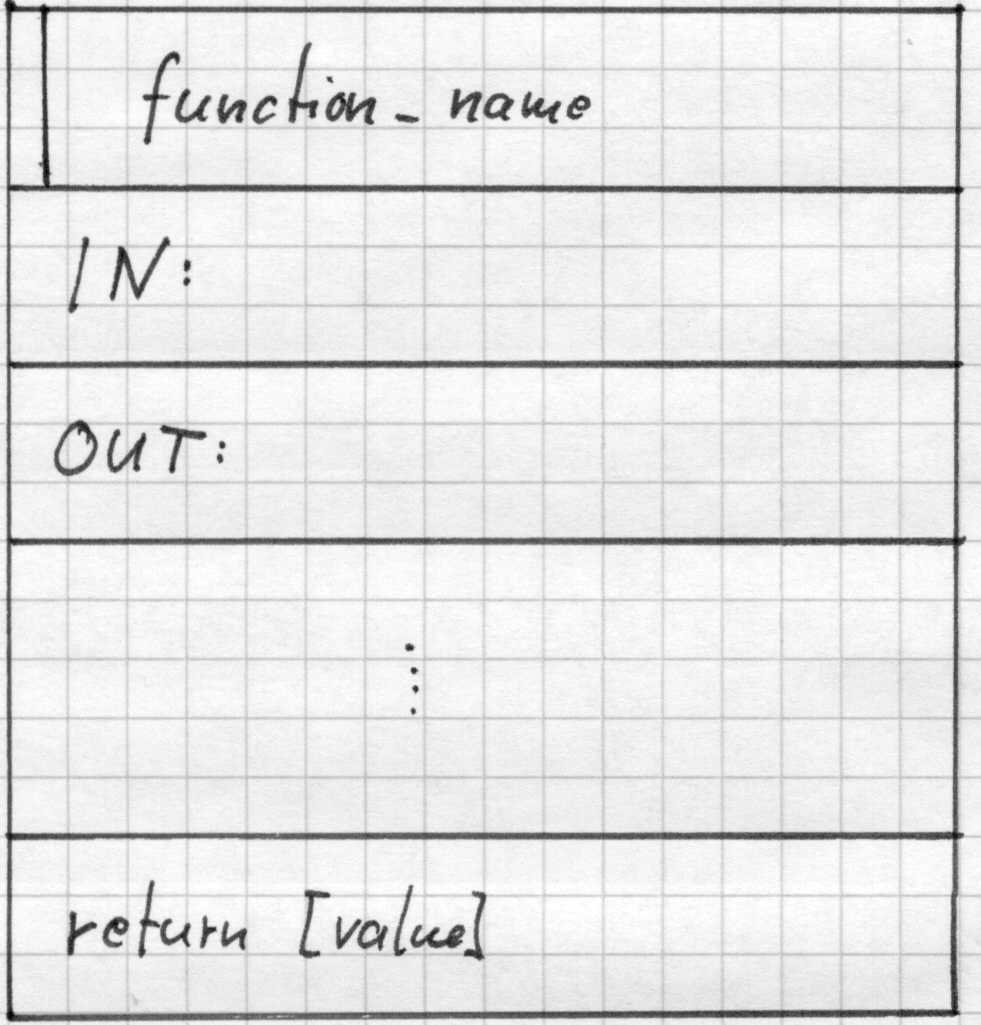
\includegraphics[scale=0.55]{GIF/p69}
%
\\
%\newpage
\textbf{Beispiel}: Wir schreiben die Berechnung von
$\text{sgn}(x)$ von Seite~\pageref{bsp:sgn1} als Funktion.\index{Signum}
%
%\includecode[linerange={6-26,33-34}]{Ex550.cpp}{Typvereinbarungen}
\includecode[firstline=6]{Ex710.cpp}{Funktion \texttt{sgn} }
%
\underline {Bemerkungen:}
 Die Funktion \verb|sgn()| ist durch ihre Signatur eindeutig beschrieben.
 Dies hat f"ur Deklaration und Definition von Funktionen die Konsequenzen:
\begin{enumerate}
 \renewcommand {\labelenumi}{(\roman{enumi})}
 \item Einige weitere (oder noch mehr) identische Funktionsdeklarationen

	\verb|double sgn(double x);|

 	sind in obigem Beispiel erlaubt.
 \item Zus"atzliche Funktionsdeklarationen mit anderen Parameterlisten
 	sind erlaubt, z.B.:\index{Funktion!Parameter|see{Parameter}}

	\verb|double sgn(double* x);| \\
	\verb|double sgn(int x);|

	da sich die Argumente von der Ausgangsdefinition unterscheiden.
	Allerdings  haben wir diese neuen Funktionen noch nicht
	definiert.
 \item  Eine zus"atzliche Deklaration %(siehe \S~\ref{sec:7.2})

	\verb|double sgn(double& x);|

	ist nicht erlaubt, da die Signatur wie unter (i) ist.
	Daher kann der Compiler nicht herausfinden,
	ob  die Funktion unter~(iii) oder die Funktion unter~(i)
	in der  Anweisung

	\verb|y = sgn(x);|

	gemeint ist.
 \item Verschiedene Funktionen mit gleichem Namen werden anhand
 	ihrer unterschiedlichen Parameterlisten identifiziert, siehe
	Pkt.~(iii).
 \item Der R"uckgabewert einer Funktion kann nicht zu ihrer
 	Identifikation herangezogen werden, die Deklarationen

	\verb|double sgn(int x);| \\
	\verb|   int sgn(int x);|

	k"onnen nicht unterschieden werden (gleiche Signatur) und daher lehnt
	der Compiler diesen Quelltext ab.
	\index{Funktion!Signatur|)}
\end{enumerate}
%
%
%
\section{Parameter"ubergabe}
\label{p:7.2}
%
Beim Programmentwurf unterscheiden wir drei Arten von Parametern einer
Funktion:
\begin{description}
 \item[INPUT] Parameterdaten werden in der Funktion benutzt aber nicht ver"andert,
 	d.h., sie sind innerhalb der Funktion \underline{konstant}.
 \item[INOUT] Parameterdaten werden in der Funktion benutzt und ver"andert.
 \item[OUTPUT] Parameterdaten werden in der Funktion initialisiert
 	und gegebenenfalls ver"andert.
\end{description}
Wir werden programmtechnisch nicht zwischen INOUT-  und OUTPUT-Parametern
unterscheiden.
%
Es gibt generell drei M"oglichkeiten
\bspfile{Ex721.cpp}
der programmtechnischen "Ubergabe von Parametern
\begin{enumerate}
  \item "Ubergabe der Daten einer Variablen (engl.: by value).
  \item "Ubergabe der Adresse einer Variablen (engl.: by address)
  \item "Ubergabe der Referenz auf eine Variable (engl.: by reference),
  	wobei hierbei versteckt eine Adresse "ubergeben wird.
\end{enumerate}
%
% \begin{latexonly}
%\begin{sidewaystable}
%\begin{landscape}      %% 2024-03-22
%
Wir betrachten die M"oglichkeiten der Parameter"ubergabe
 am Beispiel der \verb|sgn| Funktion mit der Variablen
\verb| double a |.
%\\[2ex]
%\mbox{}\hspace{-1.5cm}
\begin{table}[hbt]
\begin{tabular}{ @{\hspace{-1.5cm}}l || r | c || l | l || c | l }
 &&  & \multicolumn{2}{c||}{Effekt von} && \\
 "Ubergabeart & Parameterliste &  Aufruf
 & \verb|x++| & \verb|(*x)++| & Verwendung & Empfehlung\\ \hline\hline
%
 	& \verb|double x| & & intern & ---- & \textbf{I}NPUT & \\ \cline{2-2}\cline{4-7}
 \raisebox{1.5ex}[-1.5ex]{by value/copy}
 	& \verb|const double x| &  \raisebox{1.5ex}[-1.5ex]{\texttt{sgn(a)}}
	& nicht erlaubt & ---- & \textbf{I}NPUT & [einfache Datentypen] \\ \hline\hline
%
%
 & \verb|double& x| &  & intern/extern & ---- &
 	IN\textbf{O}UT & C++  \\ \cline{2-2}\cline{4-7}
 \raisebox{1.5ex}[-1.5ex]{by reference} & \verb|const double& x|
 	& \raisebox{1.5ex}[-1.5ex] {{\tt sgn(a)}} & nicht erlaubt & ---- &
 	\textbf{I}NPUT & C++  [komplexe Datent.] \\
     	\hline\hline
%%
 	& \verb|double* x| & 	 & intern & intern/extern &
 	IN\textbf{O}UT & \\ \cline{2-2}\cline{4-7}
 by address & \verb|const double* x| & \verb|sgn(&a)| & intern & nicht erlaubt &
 	\textbf{I}NPUT & [komplexe Datentypen] \\ 
 	\cline{2-2}\cline{4-7}
 	& \verb|double* const x| & 	& nicht erlaubt & intern/extern &
 	IN\textbf{O}UT &   \\ 
\cline{2-2}\cline{4-7}
 	& \verb|const double* const x| & 	& nicht erlaubt & nicht erlaubt &
 	\textbf{I}NPUT &  \\
  \hline
\end{tabular}
\index{Parameter!const}\index{Parameter!by reference}\index{Parameter!by value}
\index{Parameter!by address}
\caption{M\"oglichkeiten der Parameter\"ubergabe\label{tab:parameter}}
\end{table}
%
\mbox{}\\[1ex]
Die ''by-reference''-Variante \verb|double &const x|
wird vom Compiler abgelehnt.
%und die ''by-address''-Variante \verb| const double* const x |, d.h.,Zeiger und Daten d"urfen lokal nicht ver"andert werden, ist praktisch bedeutungslos.
%\end{sidewaystable}
%\end{landscape} %% 2024-03-22
% \end{latexonly}
%			sidewaystable kann fr latex2html nicht verwendet werden
% \begin{htmlonly}
% %\begin{sidewaystable}
% %
% Wir betrachten die M"oglichkeiten der Parameter"ubergabe
%  am Beispiel der \verb|sgn| Funktion mit der Variablen
% \verb| double a |.
% \\[2ex]
% %%\mbox{}\hspace{-3cm}
% %\begin{table}
% \begin{tabular}{ l || r | c || l | l || c | l }
%  &&  & \multicolumn{2}{c||}{Effekt von} && \\
%  "Ubergabeart & Parameterliste &  Aufruf
%  & \verb|x++| & \verb|(*x)++| & Verwendung & Empfehlung\\ \hline\hline
% %
%  	& \verb|double x| & & intern & ---- & \textbf{I}NPUT & [C] \\ \cline{2-2}\cline{4-7}
%  \raisebox{1.5ex}[-1.5ex]{by value}
%  	& \verb|const double x| &  \raisebox{1.5ex}[-1.5ex]{\texttt{sgn(a)}}
% 	& nicht erlaubt & ---- & \textbf{I}NPUT & C [einfache Datentypen] \\ \hline\hline
% %
%  	& \verb|double* x| & 	 & intern & intern/extern &
%  	IN\textbf{O}UT & C \\ \cline{2-2}\cline{4-7}
%  by address & \verb|const double* x| & \verb|sgn(&a)| & intern & nicht erlaubt &
%  	\textbf{I}NPUT & C [komplexe Datentypen] \\ \cline{2-2}\cline{4-7}
%  	& \verb|double* const x| & 	& nicht erlaubt & intern/extern &
%  	IN\textbf{O}UT & [C]  \\ \hline\hline
% %
%  & \verb|double& x| &  & intern/extern & ---- &
%  	IN\textbf{O}UT & C++  \\ \cline{2-2}\cline{4-7}
%  \raisebox{1.5ex}[-1.5ex]{by reference} & \verb|const double& x|
%  	& \raisebox{1.5ex}[-1.5ex]{\texttt{sgn(a)}} & nicht erlaubt & ---- &
%  	\textbf{I}NPUT & C++  \\ \hline
% \end{tabular}
% \caption{M\"oglichkeiten der Parameter\"ubergabe\label{tab:parameter}}
% %\end{table}
% %
% \mbox{}\\[1ex]
% Die ''by-reference''-Variante \verb|double &const x|
% wird vom Compiler abgelehnt und
% die ''by-address''-Variante \verb| const double* const x |, d.h.,
% Zeiger und Daten d"urfen lokal nicht ver"andert werden,
% ist praktisch bedeutungslos.
% %\end{sidewaystable}
% \end{htmlonly}

\begin{samepage}
\underline{Bemerkung zu \texttt{const}:}
\\[0.5ex]
 Wenn eine Variable in der Funktion als Konstante ben"utzt wird,
 	dann sollte  sie  auch so behandelt werden, d.h.,
	reine INPUT-Parameter sollten stets als \verb|const|\index{const}
	in der Parameterliste gekennzeichnet werden.
	Dies erh"oht die Sicherheit vor einer unbeabsichtigten
	Datenmanipulation und erleichtert auch eine sp"atere Fehlersuche.
\end{samepage}
%
%

\noindent
\underline{Bemerkung zur Äquivalenz von Pointern und Referenzen:}\\[0.5ex]
Eine Referenz \verb|double& x| entspricht dem konstanten Pointer \verb|double* const px| welcher 
nicht verändert werden kann aber über \verb|*px| kann auf den Wert im Speicher zugegriffen werden.
Dementsprechend sind in Tab.~\ref{tab:parameter} die folgenden Einträge der Parameterliste identisch:
\index{Zeiger!Referenz}\index{Referenz!Zeiger}
\\[1ex]
\begin{tabular}{lcl}
  \verb|double& x|   & $\equiv$ &  \verb|double* const px| \\
  \verb|const double& x|   & $\equiv$ &  \verb|const double* const px|
\end{tabular}

%
%
\section{R"uckgabewerte von Funktionen}
\label{p:7.3}
%
Jede Funktion besitzt ein Funktionsergebnis vom Datentyp \verb| <typ> |.
Als Typen  d"urfen verwendet werden:\index{Funktionsergebnis}
\begin{itemize}
 \item einfache Datentypen (\S~\ref{p:2.2}),
 \item Strukturen (\S~\ref{p:5.2}), Klassen,
 \item Zeiger (\S~\ref{p:6.2}),
 \item Referenzen (\S~\ref{p:6.1}),
\end{itemize}
jedoch keine C-Felder und Funktionen - daf"ur aber Zeiger auf ein Feld bzw.\
eine Funktion und Referenzen auf Felder.

Der R"uckgabewert  (Funktionsergebnis) wird mit

\verb|return <ergebnis> ;|

an das rufende Programm "ubergeben.
Ein Spezialfall sind Funktionen der  Art
\index{Funktionsergebnis!void}\index{void}

\verb|void f(<parameter_liste>)|

f"ur welche kein R"uckgabewert (void~=~leer) erwartet wird, soda"s mit

\verb|return ;|

in das aufrufende Programm zur"uckgekehrt wird.
%\includecode[linerange={6-26,33-34}]{Ex550.cpp}{Typvereinbarungen}
%\begin{samepage}
\includecode[firstline=7]{Ex731.cpp}{Funktionsergebnisse}
%\end{samepage}

\begin{samepage}
Beispiele f"ur Funktionsergebnisse:
\\
\begin{tabular}{l@{\qquad}p{0.6\textwidth}}
 \mbox{}\\
 \verb|float f1| 	    & \texttt{float}-Zahl \\[0.5ex]
 \verb|vector<float> f2| 	    & Vektor mit \texttt{float} als Elemente \\[0.5ex]
 \verb|Student f3| 	& Klasse/Struktur Student \\[0.5ex]
 \verb|vector<Student> f4| 	& Vektor mit Studenten als Elemente \\[0.5ex]
 \verb|Student* f5| 	& Zeiger auf eine Instanz der Klasse Student \\[0.5ex]
 \verb|Student& f6| 	& Referenz auf eine Instanz der Klasse Student  
  \\ & 
    \qquad entspricht\qquad \verb|Student* const f6|\\[0.5ex]
 \verb|vector<Student>& f7| 	& Referenz auf Vektor mit Studenten \\[0.5ex]
 \verb|int* f8| 	    & Zeiger auf \texttt{int}-Zahl \\[0.5ex]
 \verb|int (*f9)[]| 	& Zeiger auf C-Array von  \texttt{int}-Zahlen \\[0.5ex]
 \verb|int (*fA)()| 	& Zeiger auf Funktion, welche den Ergebnistyp \texttt{int} besitzt
 \label{fkt:f6}
\end{tabular}
\end{samepage}

\underline{Bemerkungen:}
\\[0.5ex]
 Eine Funktion darf mehrere R"uckgabeanweisungen
 \verb|return [<ergebnis>];|
 besitzen, z.B., in jedem Zweig einer Alternative eine.
 Dies ist jedoch kein sauber strukturiertes Programmieren mehr.
 \\
 $\Longrightarrow$ Jede Funktion sollte genau eine \verb|return|-Anweisung
 am Ende des Funktionsk"orpers besitzen (Standard f"ur das Praktikum).

Wie in \S\ref{p:4.8} gilt auch hier, da"s ein erfahrener Programmierer, 
also Sie noch nicht, 
unter Verwendung mehrerer \verb|return|-Anweisungen
eine Codebeschleunigung erzielen kann.
%
%
\section{Vektoren als Parameter}
\label{p:7.4}
%
%
Statische C++-Vektoren, also \texttt{array<T,N>}  k"onnen analog zu ihrer Deklaration als Funktionsparameter
"ubergeben werden. Allerdings m"ussen alle Dimensionen zum Compilierungszeitpunkt bekannt sein.
\index{Parameter!Feld}\index{Parameter!Vektor}\index{Vektor}

Wir betrachten als erstes \textbf{Beispiel} die Ausgabe eines
Vektors,
d.h., Vektors $\underline{x}$ der L"ange~$n$.
%

% \pagebreak[4]
\underline{Struktogramm}: \\
%\begin{latexonly}
%  \special{psfile=GIF/p71.eps.gz
%	   hscale=15 vscale=15
%	   voffset=-135
%	  }
%  \vspace{5cm}
%\end{latexonly}
%\htmladdimg{p71_4.jpg}{}
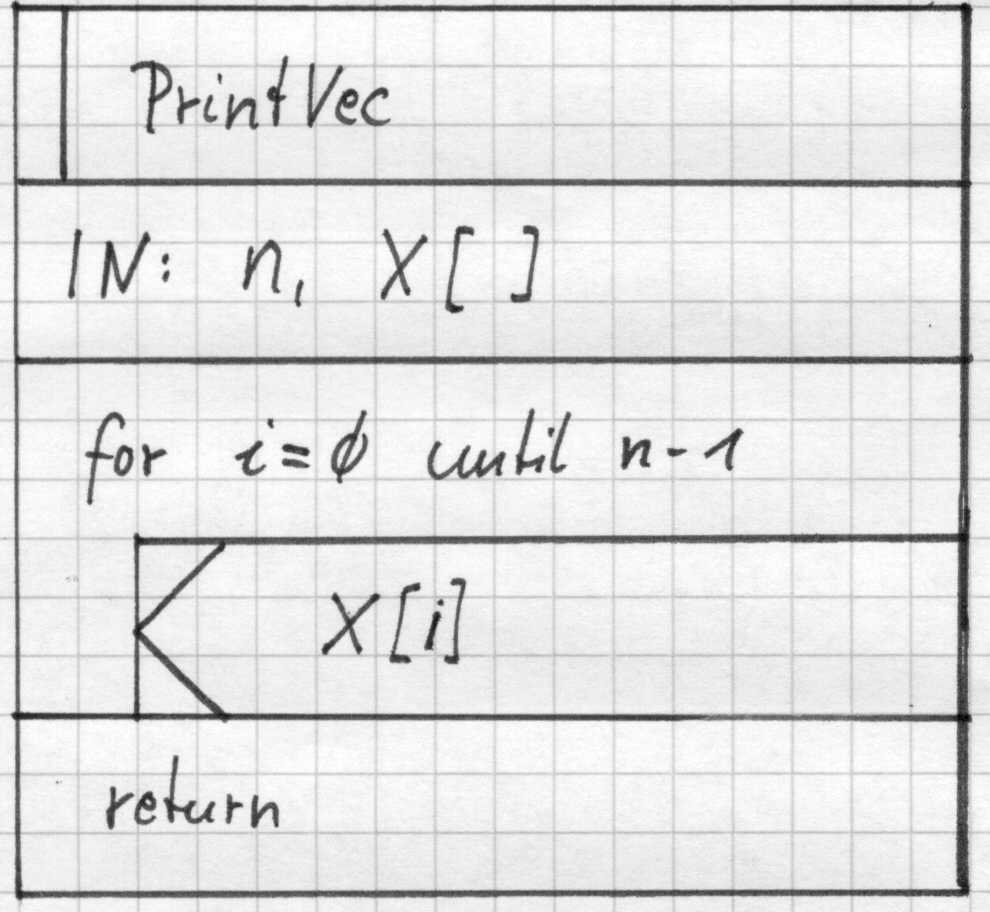
\includegraphics[scale=0.7]{GIF/p71}
%
\includecode[linerange={7-8,11-13,15-19,38-48,93-94,112-117}]{bsp740.cpp}{Vektor als Parameter}
%

Als n"achstes betrachten wir die Ausgabe eines statischen 2D-Feldes,
d.h., einer Matrix mit \verb|MCOL|~Spalten und \verb|NROW|~Zeilen.
Hier \textbf{mu"s} die Anzahl der Spalten als globale Konstante definiert
werden, da ansonsten die nachfolgende Funktion nicht compiliert werden kann.
\index{Parameter!Matrix}\index{Matrix}\index{Feld!statisch}
%
\includecode[linerange={7-9,10-13,22-26,57-70,93-98,108-108,116-117},label=lst:bsp740.cpp_b]{bsp740.cpp}{Matrix als Parameter}
%

Leider k"onnen wir die Funktion \verb|PrintMat_fix| nur f"ur
statische 2D-Felder (Matrizen) anwenden, und dann auch nur f"ur
solche mit \verb|NCOL=3| Spalten - schon eine Matrix
\verb|double aa[7][9]| kann mit dieser Funktion nicht mehr ausgegeben
werden.
Jedoch k"onnen wir das 2D-Feld als 1D-Feld der L"ange \verb|NROW*MCOL|
auffassen und so die Funktion dahingehend verallgemeinern, da"s
beliebige statische 2D-Felder und als 2D-Felder interpretierbare
dynamische 1D-Felder
(wie in Version~2 auf Seite~\pageref{page:2DarrayVariant2})
"ubergeben werden k"onnen. Diese Funktion kann beliebigen Zeilen- und Spaltenanzahlen arbeiten.
% exfile{Ex740.cpp}
\index{Parameter!Matrix}\index{Matrix}\index{Feld!dynamisch}
%
\includecode[linerange={7-13,29-35,76-89,93-95,101-105,109-109,117-119},label=lst:Ex740.cpp_c]{bsp740.cpp}{Dynamischer Vektor als Parameter interpretiert als Matrix}
%

Eine komfortable Lösung der Übergabe einer Matrix als Parameter besteht darin, 
daß man eine Klasse~\texttt{Matrix} deklariert welche alle notwendige Funktionalität 
enthält~\S\ref{p:9}.
%
%   OLD: C-Teil
%
\ifcteil
%\newpage{}
\section{Vektoren als Parameter}
\label{sec:7.4}
%
\textbf{\Large  Analog wie nächster Abschnitt, nur mit vector<> !! \\
Verweis auf Klasse Matrix später}
%
\section{\mbox{}$^{*}$C-Array als Parameter}
\label{sec:7.4}
%
%
Statische Felder k"onnen analog zu ihrer Deklaration als Funktionsparameter
"ubergeben werden. Allerdings m"ussen alle Dimensionen, au"ser der
h"ochsten Dimension, zum Compilierungszeitpunkt bekannt sein.
\index{Parameter!Feld}\index{Parameter!Vektor}\index{Vektor}

Wir betrachten als erstes \textbf{Beispiel} die Ausgabe eines
(statischen oder dynamischen) 1D-Feldes,
d.h., Vektors $\underline{x}$ der L"ange~$n$.
%

% \pagebreak[4]
\underline{Struktogramm}: \\
%\begin{latexonly}
%  \special{psfile=GIF/p71.eps.gz
%	   hscale=15 vscale=15
%	   voffset=-135
%	  }
%  \vspace{5cm}
%\end{latexonly}
%\htmladdimg{p71_4.jpg}{}
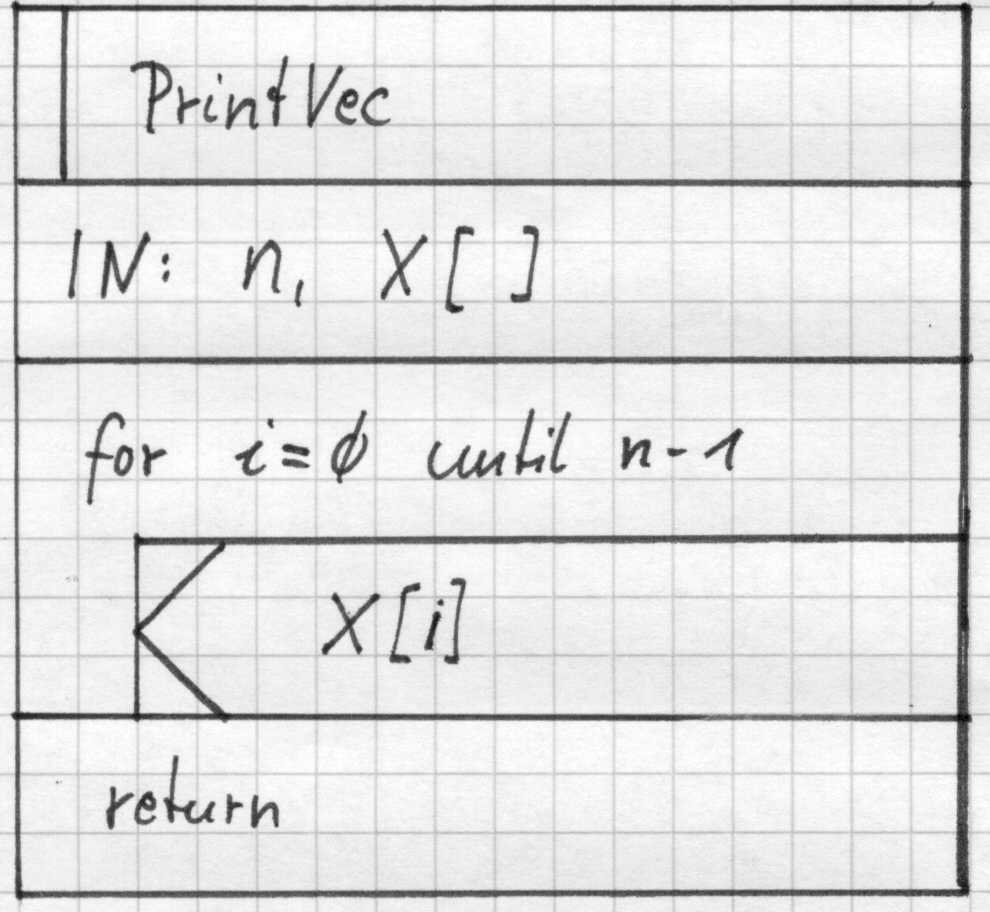
\includegraphics[scale=0.7]{GIF/p71}
%
\includecode[linerange={7-10,13-18,42-51,94-94,115-116,118-119}]{Ex740.cpp}{C-Array als Parameter}
%

Als n"achstes betrachten wir die Ausgabe eines statischen 2D-Feldes,
d.h., einer Matrix mit \verb|MCOL|~Spalten und \verb|NROW|~Zeilen.
Hier \textbf{mu"s} die Anzahl der Spalten als globale Konstante definiert
werden, da ansonsten die nachfolgende Funktion nicht compiliert werden kann.
\index{Parameter!Matrix}\index{Matrix}\index{Feld!statisch}
%
\includecode[linerange={7-10,21-27,59-72}]{Ex740.cpp}{2D-Array als Parameter}
%

Leider k"onnen wir die Funktion \verb|PrintMat_fix| nur f"ur
statische 2D-Felder (Matrizen) anwenden, und dann auch nur f"ur
solche mit \verb|NCOL=3| Spalten - schon eine Matrix mit 4 Spalten 
kann mit dieser Funktion nicht mehr ausgegeben
werden.
Jedoch k"onnen wir das 2D-Feld als 1D-Feld der L"ange \verb|NROW*MCOL|
auffassen und so die Funktion dahingehend verallgemeinern, da"s
beliebige statische 2D-Felder und als 2D-Felder interpretierbare
dynamische 1D-Felder
(wie in Version~2 auf Seite~\pageref{page:2DarrayVariant2})
"ubergeben werden k"onnen. 
% exfile{Ex740.cpp}
\index{Parameter!Matrix}\index{Matrix}\index{Feld!dynamisch}
%
\includecode[linerange={7-10,30-37,78-90,74-112,117-119}]{Ex740.cpp}{Dynamisches C-Array as Parameter interpretiert als Matrix}
%

Da die Funktion \verb|PrintMat|
\enlargethispage{4ex}
ein 1D-Feld erwartet (also ein Zeiger),
mu"s vom statischen 2D-Feld \verb|a| ein Zeiger auf die erste
Zeile der Matrix "ubergeben werden.
Daher erscheint \verb|a[0]| in der entsprechenden Rufzeile.
\fi{}
%
%   OLD - ende
%
%
%	Header files
%
\section{Deklarationen und Headerfiles, Bibliotheken}
\label{p:7.5}
%\textbf{\Large  Alle Beispiele mit C++-Vektoren}
%
Normalerweise setzt sich der Quelltext eines Computerprogrammes aus
(wesentlich) mehr als einem Quelltextfile zusammen. Damit Funktionen,
Datenstrukturen (und globale Konstanten, Variablen) und Makros
aus anderen Quelltextfiles (\textit{name.cpp})
genutzt werden k"onnen, benutzt man
\textbf{Headerfiles} (\textit{name.h}, \textit{name.h}) welche als \textbf{"offentliche Schnittstelle}
die Deklarationen f"ur die Funktionen des  Quelltextfiles \textit{name.cpp}
(=~versteckter Bereich) beinhalten.
Sie dazu \cite[\S8.1]{Wolf:2006:CAZ}.
\index{Funktion!Deklaration}\index{Headerfile}\index{Bibliothek}\index{Quellfile}
\\[-4ex]
\enlargethispage{3ex}
%
%
\subsection{Beispiel: \texttt{printvec}}
\label{p:7.5.1}
%
Wir wollen die in \S\ref{p:7.4} programmierten Funktionen
\texttt{PrintVec} und \texttt{PrintMat} in einem anderen Quelltext
(d.h., Hauptprogramm) benutzen.
Zun"achst kopieren wir die Definitionen der beiden Funktionen
(und alles andere, was zum Compilieren ben"otigt wird) in
das neue File \textit{printvec.cpp}.\bspfile{printvec.cpp}
%
\begin{lstlisting}[caption=Implementierungsteil der Print-Funktionen,label=lst:7_6_1,basicstyle=\scriptsize]{}
#include <iostream>
#include <vector>
#include <cassert>                      // assert()
using namespace std;

void PrintVec(const vector<double> &x)
{
    ...
}

void PrintMat(const int nrow, const int ncol, const vector<double> &a)
{
    assert(nrow*ncol==a.size());        // sind die Parameter kompatibel?
    ...
}
\end{lstlisting}
%
Die C-Funktion \texttt{assert()} erwartet eine Wahrheitswert als Inputparameter 
und bricht die Abarbeitung des Programmes sofort ab, falls dieser \texttt{false} ist.
Da hierbei Name und Zeilennummer des Quelltextfiles angegeben werden, ist die Funktion
\texttt{assert()} eine einfache Möglichkeit, um die Zulässigkeit bestimmter Größen zu überprüfen.
Der Test läßt sich mit der Compileroption \texttt{-DNDEBUG} bequem ausschalten.
Die C++-Fehlerbehandlung über das \emph{exception handling} ist komplexer,
für unsere Zwecke auch noch nicht nötig und
wird im Rahmen der der LV nicht behandelt.

Das File \textit{printvec.cpp} wird nun compiliert (ohne es zu linken!)
\\[0.5ex]
\verb| LINUX> g++ -c -Wall -pedantic printvec.cpp |
\\[0.5ex]
wodurch das Objektfile \textit{printvec.o} erzeugt wird.

Das Hauptprogramm in \mbox{\textit{Ex751-old.cpp}}
%\bspfile{Ex751-old.cpp}
ben"otigt nunmehr die Deklarationen der beiden Funktionen.

%\includecode[linerange={7-10,30-37,78-90,74-112,117-118}]{Ex751-old.cpp}{Hauptprogramm ohne Headerfile}
\includecode[firstline=10]{Ex751-old.cpp}{Hauptprogramm ohne Headerfile}
%
Das  Compilieren des Hauptfiles
\\[0.2ex]
\verb| LINUX> g++ -c -Wall -pedantic Ex751-old.cpp |
\\[0.2ex]
erzeugt das Objektfile \textit{Ex751-old.o} welches
mit dem anderen Objektfile zum fertigen Programm \textit{a.out}
gelinkt werden mu"s
\\[0.2ex]
\verb| LINUX> g++ Ex751-old.o printvec.o |
\\[0.2ex]
S"amtliches compilieren und linken l"a"st sich auch in einer
Kommandozeile ausdr"ucken
\\[0.2ex]
\verb| LINUX> g++ -Wall -pedantic Ex751-old.cpp printvec.cpp |
\\[0.2ex]
wobei manche Compiler im ersten Quelltextfile (hier \textit{Ex751-old.cpp})
das Hauptprogramm \texttt{main()} erwarten.

Die Deklarationen im Hauptprogramm  f"ur die Funktionen aus
\textit{printvec.cpp} schreiben wir in das Headerfile
\textit{printvec.h}

%\includecode[linerange={7-10,30-37,78-90,74-112,117-118}]{printvec.h}{Header der Print-Funktionen}
\includecode[firstline=4]{printvec.h}{Header der Print-Funktionen}

und wir ersetzen den Deklarationsteil im Hauptprogramm durch die
Pr"aprozessoranweisung
\\[0.2ex]
\verb|#include "printvec.h"|
\\[0.2ex]
welche den Inhalt \textit{printvec.h} vor dem Compilieren von
\textit{Ex751.cpp} \bspfile{Ex751.cpp}
automatisch einf"ugt.

\begin{lstlisting}[caption=Hauptprogramm mit Headerfile,label=lst:7_6_4,basicstyle=\scriptsize]{}
#include <vector>
using namespace std;
//			declarations of functions from printvec.cpp
#include "printvec.h"

int main()
{
    ...
}
\end{lstlisting}
Die Anf"uhrungszeichen  \verb| "  " |  um den Filenamen
kennzeichnen, da"s das Headerfile \textit{printvec.h}
im gleichen Verzeichnis wie das Quelltextfile \textit{Ex751.cpp}
zu finden ist.

\begin{minipage}{\textwidth}
Das Kommando
\\[0.2ex]
\verb| LINUX> g++ -Wall -pedantic Ex751.cpp printvec.cpp |
\\[0.2ex]
erzeugt wiederum das Programm \textit{a.out}.
\end{minipage}
%
%
%\pagebreak
%\newpage
\subsection{Beispiel: \texttt{student}}
\label{p:7.5.2}
%
Wir k"onnen auch selbstdefinierte Datenstrukturen, z.B.
die Datenstrukturen \texttt{Student}, \texttt{Student\_Mult}
aus~\S\ref{p:5.3} 
%und  \texttt{Student2} aus \S\ref{sec:6.4}
und globale Konstanten
in einem Headerfile \textit{student.h} speichern.
%\bspfile{student.h}
\index{Student}\index{Student!Student2}
%\includecode[linerange={7-10,30-37,78-90,74-112,117-118}]{student.h}{Header der Strukturen und der Funktion}
\includecode[firstline=2]{student.h}{Header der Strukturen und der Funktion}
%
%
Die neue Funktion \texttt{Copy\_Student} wird in
\textit{student.cpp} definiert,
wobei der Funktionsk"orper aus \textit{Ex643-correct.cpp} kopiert wurde.
%\includecode[linerange={7-10,30-37,78-90,74-112,117-118}]{student.h}{Header der Strukturen und der Funktion}
\includecode[firstline=4]{student.cpp}{Implementierung der Funktion welche die neuen Strukturen nutzt}
%
Da die Struktur \texttt{Student} verwendet wird, mu"s auch das
Headerfile \textit{student.h} in \textit{student.cpp} eingebunden werden.
Die neue Funktion \texttt{Copy\_Student} kann nunmehr im Hauptprogramm
\textit{bsp752.cpp} \bspfile{bsp752.cpp} zum Kopieren einer Struktur auf eine andere
benutzt werden. Das Hauptprogramm ben"otigt daf"ur nat"urlich wieder
das Headerfile \textit{student.h}.

Das Kommando
\\[0.2ex]
\verb| LINUX> g++ -std=c++11 -Wall -pedantic bsp752.cpp student.cpp  |
\\[0.2ex]
erzeugt schlu"sendlich das Programm \textit{a.out}.
\\ \vfill\mbox{}
%
%
\subsection{Eine einfache Bibliothek am Beispiel \texttt{student}}
\label{p:7.5.3}
%
Um sich das wiederholte compilieren zus"atzlicher Quelltextfiles
und die damit verbundenen u.U.\  langen Listen von Objektfiles
beim Linken zu ersparen, verwendet man Bibliotheken.
Gleichzeitig haben Bibliotheken den Vorteil, da"s man seine
compilierten Funktionen (zusammen mit den Headerfiles) anderen in kompakter
Form zur Verf"ugung stellen kann, ohne da"s
man seine Programmiergeheimnisse (geistiges Eigentum) verraten mu"s.
Dies sei an hand des (sehr einfachen) Beispiels aus \S\ref{p:7.5.2}
demonstriert.
\index{Bibliothek}\index{Student!Bibliothek}
\begin{itemize}
 \item Erzeugen des Objektfiles \textit{student.o} (compilieren)
    \index{Quellfile!compilieren}
    \\[0.2ex]
    \verb| LINUX> g++ -c student.cpp |
%    \\[0.2ex]
 \item Erzeugen/Aktualisieren der Bibliothek \textit{lib\underline{stud}.a}
 	(archivieren) aus/mit dem Objektfile  \textit{student.o}.
	Der Bibliotheksbezeichner \underline{stud} ist frei w"ahlbar.
	\index{Bibliothek!erzeugen}\index{Bibliothek!aktualisieren}
    \\[0.2ex]
    \verb| LINUX> ar r libstud.a student.o|
    \\[0.2ex]
    Die Archivierungsoptionen (hier, nur \verb|r|) k"onnen mit
    dem verwendeten Compiler variieren.
 \item Compilieren des Hauptprogrammes \bspfile{bsp752.cpp} und
       linken mit der Bibliothek aus dem aktuellen Verzeichnis
       \index{Linken}\index{Bibliothek!linken}
    \\[0.2ex]
    \verb| LINUX> g++ bsp752.cpp -L. -lstud|
%    \\[0.2ex]
\end{itemize}
%

%%\fbox {
%%\begin{minipage}{0.98\textwidth}
%
Die folgenden Schritte sind notwendig, um das Programm ohne
Verwendung einer Bibliothek zu \"ubersetzen und zu linken.
\index{Compilieren!g++}
\[
\begin{CD}
  \left.
  \begin{CD}
   \textit{student.cpp} @>\texttt{g++ -c student.cpp}>> \textit{student.o}
   \\
   \textit{bsp752.cpp} @>\texttt{g++ -c bsp752.cpp}>> \textit{bsp752.o}
  \end{CD}
  \right\}
  @>\texttt{g++ bsp752.o student.o}>> \textit{a.out}
\end{CD}
\]
Abk\"urzend ist auch m\"oglich:
\[
  \begin{CD}
   \textit{bsp752.cpp, student.cpp} @>\texttt{g++ bsp752.cpp student.cpp}>> \textit{a.out}
  \end{CD}
\]
Bei Verwendung der Biobliothek \textit{lib}\textbf{stud}\textit{.a} sieht der
Ablauf folgenderma{\ss}en aus
\[
\begin{CD}
  \left.
  \begin{CD}
   \textit{student.cpp} @>\texttt{g++ -c }>\texttt{student.cpp}> \textit{student.o}
   @>\texttt{ar r lib}\textbf{stud}\texttt{.a }>\texttt{student.o}>
   \textit{lib}\textbf{stud}\textit{.a}
   \\
   \textit{bsp752.cpp} @>\texttt{g++ -c }>\texttt{bsp752.cpp}> \textit{bsp752.o}
  \end{CD}
  \right\}
  @>\texttt{g++ bsp752.o}>\texttt{ -L. -l}\textbf{stud}> \textit{a.out}
\end{CD}
\]
was bei bereits vorhandener Bibliothek wiederum abgek\"urzt werden kann:
\[
\begin{CD}
   \textit{bsp752.cpp, }\textit{lib}\textbf{stud}\textit{.a}
    @>\texttt{g++ bsp752.cpp -L. -l}\textbf{stud}>> \textit{a.out}
\end{CD}
\]
%
%%\end{minipage}
%%}
%
%
%
%\pagebreak[4]
\section{Das Hauptprogramm}
\label{p:7.6}
%
\begin{minipage}[t] {0.75\textwidth}
Das Hauptprogramm\index{main()}
ist eine Funktion \verb|main| welche im gesamten Code \emph{genau einmal} auftreten darf
und von welcher ein Rückgabewert vom Typ~\verb|int| erwartet wird..
Bislang benutzen wir diese Funktion ohne Parameterliste.
Das Programm wird von einer Umgebung (meist eine \emph{Shell}) aufgerufen welche
ihrerseits diesen Rückgabewert auswerten kann. Dabei wird ein
Rückgabewert~0 als fehlerfreie Programmabarbeitung interpretiert.
\end{minipage}
\hfill
\begin{minipage}[t] {0.2\textwidth}
\begin{verbatim}
int main()
{
   ...
   return 0;
}
\end{verbatim}
\end{minipage}


Die Programmabarbeitung kann jederzeit, auch in Funktionen, mit der
Anweisung \verb|exit(<int_value>);| abgebrochen werden.
Der Wert \verb|<int_value>| ist dann der  R"uckgabewert des Programmes
und
kann zur Fehlerdiagnose herangezogen werden.
Ab der Version 4.3 des Gnu--Compilers m"ussen zus"atzliche Headerfiles f"ur
einige eingebaute Funktionen (hier f"ur \textrm{exit()} und \textrm{atoi()})
eingebunden werden, siehe die
%\htmladdnormallinkfoot{kompakte}{\url{http://www.cyrius.com/journal/gcc/gcc-4.3-include}}
\htmladdnormallinkfoot{kompakte}{http://www.cyrius.com/journal/gcc/gcc-4.3-include}
%bzw. \htmladdnormallinkfoot{ausf"uhrliche}{\url{http://gcc.gnu.org/gcc-4.3porting_to.html}}
bzw.\   \htmladdnormallinkfoot{ausf"uhrliche}{http://gcc.gnu.org/gcc-4.3/porting_to.html}
Darstellung der "Anderungen.

Das Programm in Listing~\ref{lst:Ex760.cpp} bricht bei $n < 0$ die Programmausf"uhrung
in \verb|spass()| sofort ab und liefert den Fehlercode~-10 zurück.
%

Wie bei anderen Funktionen kann auch das Hauptprogramm mit Parametern
aufgerufen werden, allerdings ist in
\index{Parameter!main()}

\centerline{\texttt{int main(int argc, char* argv[])}}

die Parameterliste (genauer, die Typen der Parameter) vorgeschrieben, wobei
\begin{itemize}
 \item \verb|argv[0]| den Programmnamen und
 	\index{argv[]}\index{argc}
 \item \verb|argv[1]| $\ldots$ \verb|argv[argc-1]| die Argumente
 	beim Programmaufruf als Zeichenketten "ubergeben.
 \item Es gilt stets \verb|argc|$\ge 1$, da der Programmname
 	immer als \verb|argv[0]| übergeben wird.
\end{itemize}
%
%\includecode[linerange={7-10,30-37,78-90,74-112,117-118}]{Ex760.cpp}{Hauptprogramm mit Parametern}
\includecode[firstline=12]{Ex760.cpp}{Hauptprogramm mit Parametern}
%

Die Funktion\index{atoi()} \verb|atoi(char *)| (=~ASCII to int)
wandelt die "ubergebene Zeichenkette in
eine Integerzahl um und wird im Header \textit{cstdlib} deklariert.
Mittels der analogen Funktion\index{atod()} \verb|atod(char *)| l"a"st sich eine
Gleitkommazahl als Parameter "ubergeben.
Nach dem Compilieren und Linken kann das Programm \verb|a.out|
mittels
\\[0.5ex] \verb|LINUX> ./a.out| \\[0.5ex] bzw.\\[0.5ex] \verb|LINUX> ./a.out 5| \\[0.5ex]
gestartet werden. Im ersteren Fall wird der Wert von \verb|n| von
der Tastatur eingelesen, im zweiten Fall wird der Wert \verb|5|
aus der Kommandozeile "ubernommen und \verb|n| zugewiesen.
Eine elegante, und echte C++-L"osung, bzgl. der "Ubergabe von
Kommandozeilenparametern kann in \cite[pp.126]{Stroustrup:2000:CPP}
gefunden werden.
%
%
\section{Rekursive Funktionen}
\label{p:7.7}
Funktionen k"onnen  in C/C++ rekursiv aufgerufen werden.
\index{Funktion!rekursiv|see{Rekursion}}\index{Rekursion!Funktion}
\\
\textbf{Beispiel}: Die Potenz $x^k$ mit $x\in {\mathbb{R}}$, $k\in {\mathbb{N}}$
kann auch als
$
x^k = \begin{cases} x\cdot x^{k-1} & k>0 \\ 1 &  k=0\end{cases}
$
realisiert werden.
\pagebreak[3]
\includecode[linerange={32-45}]{Ex770.cpp}{Rekursive Funktion~\texttt{power}}
%
%
%
\section{Ein gr"o"seres Beispiel: Bisektion}
\label{p:7.8}
%
Im\index{Bisektion|(} Beispiel auf Seite~\pageref{bsp:bisection0} ging es darum, die
Nullstelle von $f(x):=\sin(x)-x/2$ im Intervall (a,b), mit
$a=0$ und $b=1$ zu bestimmen.
Unter der Voraussetzung $f(a) > 0 > f(b)$ kann dieses Problem
(f"ur stetige Funktionen)
mittels Bisektion gel"ost werden.
Der Bisektionsalgorithmus besteht f"ur jedes Intervall $[a,b]$
im wesentlichen aus den Schritten
\begin{enumerate}
 \renewcommand {\labelenumi}{(\roman{enumi})}
 \item $c:=(a+b)/2$
 \item Ist $|f(c)|$ nah genug an $0$~?
 \item In welcher Intervallh"alfte mu"s ich weitersuchen~?
\end{enumerate}
Dies ist eine klassische Rekursion, wobei
Punkt~(iii) die n"achste Rekursion einleitet und Punkt~(ii)
den Abbruch der Rekursion garantieren soll. Formal k"onnen wir dies so
ausdr"ucken:
\index{Rekursion}\index{Rekursion!Abbruchtest}
$$
 x_0 := \text{Bisect} (a,b,\varepsilon) :=
 \begin{cases}
  c:=(a+b)/2 & \text{falls } |f(c)| < \varepsilon \\
  \text{Bisect} (c,b,\varepsilon) & \text{sonst, falls } f(c) > 0 \\
  \text{Bisect} (a,c,\varepsilon) & \text{sonst, falls } f(c) < 0 \\
 \end{cases}
$$
%
\underline{Struktogramm}: \\
%\begin{latexonly}
%  \special{psfile=GIF/p85.eps.gz
%	   hscale=20 vscale=20
%	   voffset=-290
%	  }
%  \vspace{11cm}
%\end{latexonly}
%\htmladdimg{p85_4.jpg}{}
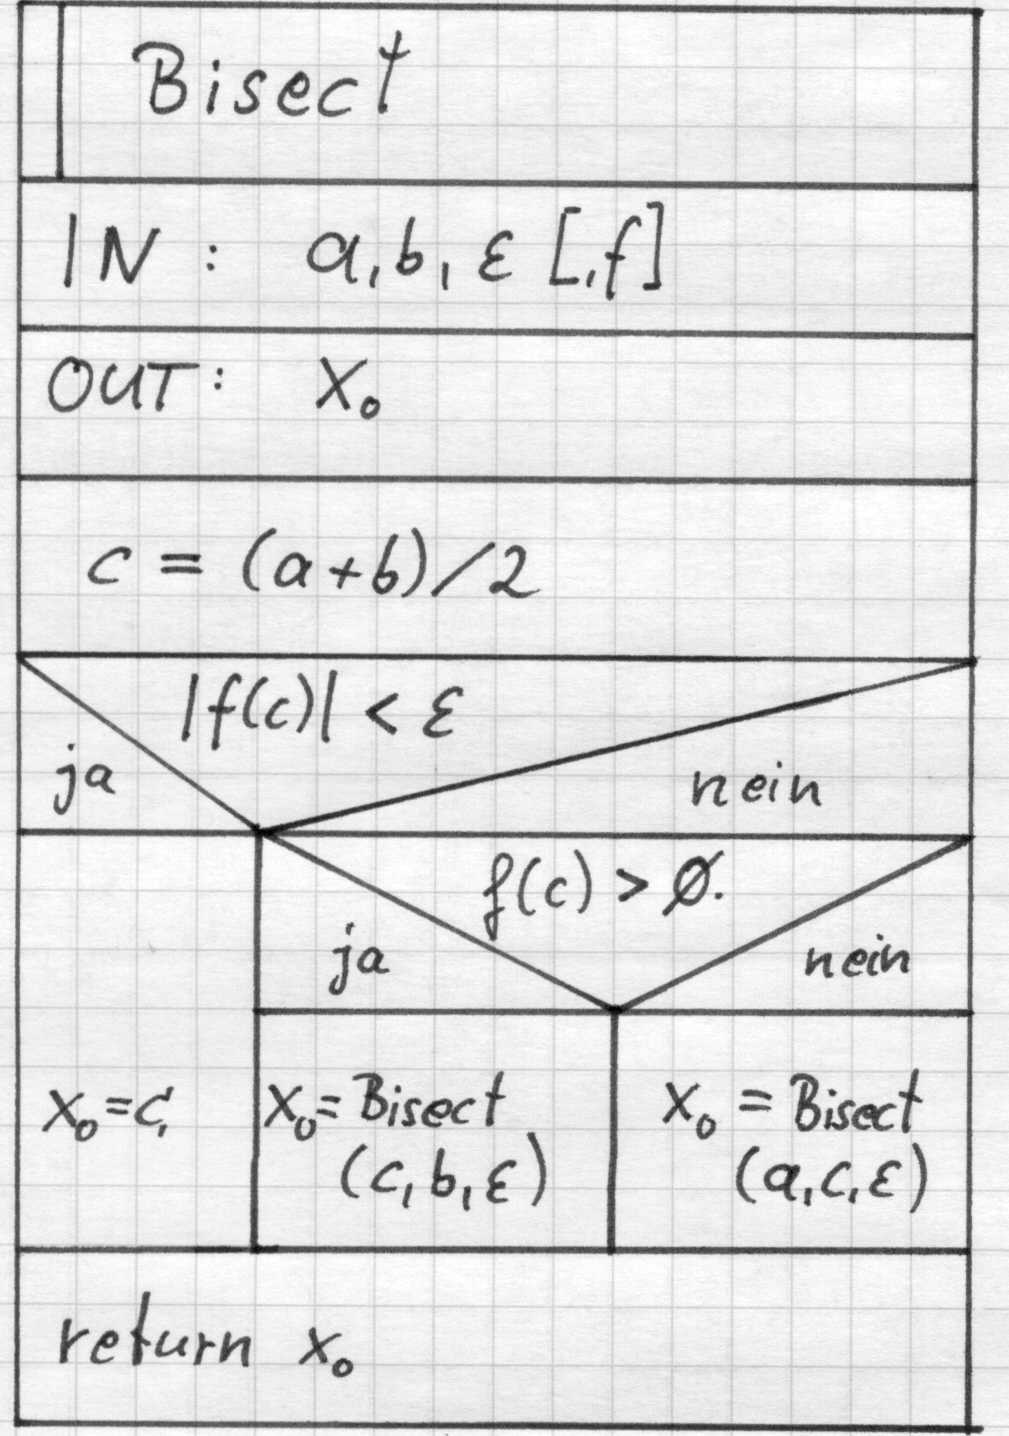
\includegraphics[scale=0.7]{GIF/p85}

Dies ergibt die Funktionsdefinition f"ur \verb|Bisect()| welche
mit
\\
\verb|    x0 = Bisect(a,b,1e-6);|
\\
aufgerufen wird und zur \underline{Version~1} des Bisektionsprogrammes f"uhrt.
%
\includecode[linerange={45-61}]{Bisect1.cpp}{Bisektion-I}
%
%\exfile{Bisect1.cpp}
%\\
%\begin{minipage} {0.999\textwidth}
%\begin{boxedverbatim}
%double Bisect1(const double a, const double b, const double eps)
%{
 %double x0, fc, c = (a+b)/2;

 %fc = sin(c) - 0.5*c;
 %if ( fabs(fc) < eps )             // end of recursion
  %{
   %x0 = c;
  %}
 %else if (  fc > 0.0 )
  %{
   %x0 = Bisect1(c,b,eps);          // search in the right intervall
  %}
 %else                              // i.e., fc < 0.0
  %{
   %x0 = Bisect1(a,c,eps);          // search in the left intervall
  %}

 %return x0;                        // return the solution
%}
%\end{boxedverbatim}
%\end{minipage}

Um das Programm etwas flexibler zu gestalten, werden wir die fix
in \verb|Bisect1()| einprogrammierte Funktion $f(x)$ durch die
globale Funktion

\begin{lstlisting}[caption=Globale Funktion und globale Konstante,label=lst:7_9_2,basicstyle=\scriptsize]{}
const double EPS = 1e-6;           // global constant

double f(const double x)           // declaration and definition of function f(x)
{
    return  sin(x) - 0.5 * x ;
}
\end{lstlisting}

%\begin{minipage} {0.999\textwidth}
%\begin{boxedverbatim}
%double f(const double x)        // declaration and
  %{ return  sin(x) - 0.5*x ; }  //   definition of function f(x)
%\end{boxedverbatim}
%\end{minipage}

ersetzen.
Gleichzeitig k"onnten wir den Funktionsparameter \verb|eps| durch eine globale
Konstante \verb|EPS| ersetzen, soda"s sich Version~II des Codes ergibt.
\bspfile{Bisect2.cpp}
\index{Konstante!globale}

Die Flexibilit"at der Bisektionsfunktion l"a"st sich weiter erh"ohen, 
indem wir die auszuwertende Funktion $f(x)$ als Variable in der
Parameterliste "ubergeben. Bei einer Funktion als Parameter müssen die Argumente 
wie die Deklaration f"ur \verb|f6| auf Seite~\pageref{fkt:f6} aufgebaut sein.
Konkret hei"st dies:
\index{Parameter!Funktion}
\\[0.5ex]
\verb|std::function<double(double)>| ist eine Typbezeichnung für eine
Funktion mit einer \verb|double|-Variablen als Argument
und \verb|double| als Typ des R"uckkehrwertes (C++11; \verb|#include <functional>|)~\cite[\S23.3.1]{Will:2018:CPT}.
\\[0.5ex]
Dies erlaubt uns die Funktionsdeklaration und -definition von
\verb|Bisect3()|.
%
\includecode[linerange={9-9,34-34,49-54,73-74,79-99}]{Bisect3.cpp}{Bisektion-III mit Funktion als Parameter}

%\begin{minipage} {0.99\textwidth}
%\begin{boxedverbatim}
               %// declaration of Bisect3
%double Bisect3(double (*func)(double), const double a,
                %const double b, const double eps=1e-6);
%...
%main()
%{...}
               %// definition of Bisect3
%double Bisect3(double (*func)(double), const double a,
                     %const double b, const double eps)
%{
 %double x0, fc, c = (a+b)/2;

 %fc = func(c);     // calculate value of parameter function
 %if ( fabs(fc) < eps )
  %{
   %x0 = c;                      // end of recursion
  %}
 %else if (  fc > 0.0 )
  %{
   %x0 = Bisect3(func,c,b,eps);  // search in right intervall
  %}
 %else                           // i.e., fc < 0.0
  %{
   %x0 = Bisect3(func,a,c,eps);  // search in left intervall
  %}

 %return x0;                     // return the solution
%}
%\end{boxedverbatim}
%\end{minipage}

Das vierte Argument (\verb|eps|) in der Parameterliste von \verb|Bisect3()|
ist ein\index{Parameter!optionales Argument} \textbf{optionales Argument}, welches
beim Funktionsaufruf nicht "ubergeben werden mu"s. In diesem Fall
wird diesem optionalen Argument sein, in der Funktionsdeklaration festgelegter,
Standardwert automatisch zugewiesen. In unserem Falle w"urde also der Aufruf
im Hauptprogramm
\\[0.5ex]
\verb|    x0 = Bisect3(f,a,b,1e-12)|
\\[0.5ex]
die Rekursion bei $|f(c)| < \varepsilon := 10^{-12}$ abbrechen,
w"ahrend
\\[0.5ex]
\verb|    x0 = Bisect3(f,a,b)|
\\[0.5ex]
schon bei $|f(c)| < \varepsilon := 10^{-6}$ stoppt.
%\exfile{Bisect3.cpp}

Wir k"onnten jetzt eine weitere Funktion
\begin{lstlisting}[caption=Weitere globale Funktion,label=lst:7_9_5,basicstyle=\scriptsize]{}
double g(const double x)           // declaration and definition of function g(x)
{
    return -(x-1.234567)*(x+0.987654) ;
}
\end{lstlisting}
%\begin{minipage} {0.99\textwidth}
%\begin{boxedverbatim}
                          %// declaration and
%double g(const double x)
                          %//   definition of function g(x)
  %{ return -(x-1.234567)*(x+0.987654) ; }
%\end{boxedverbatim}
%\end{minipage}
%
deklarieren und definieren, und den Bisektionsalgorithmus
in Version~III\bspfile{Bisect3.cpp} mit dieser aufrufen:
\\[0.5ex]
\verb|    x0 = Bisect3(g,a,b,1e-12)|
\\[0.5ex]

%\underline{Bemerkung:}
%Da unsere, als Argument in \verb|Bisect3|
%"ubergebene, Funktion \verb|func| ein reiner INPUT-Parameter ist,
%sollten wir sie noch mit \verb|const| kennzeichnen.
%Allerdings ist die korrekte Kennzeichnung des ersten Arguments in \verb|Bisect3|
%%
%\begin{lstlisting}[caption=Konstanter Funktionspointer,label=lst:7_9_6,basicstyle=\scriptsize]{}
%double Bisect3(double (* const func)(double), const double a, const double b,
               %const double eps=1e-6);
%\end{lstlisting}
%\begin{minipage} {0.99\textwidth}
%\begin{verbatim}
%double Bisect3(double (* const func)(double), const double a,
              %const double b, const double eps=1e-6);
%\end{verbatim}
%\end{minipage}

%
%anfangs etwas verwirrend.

Unser Programm
arbeitet zufriedenstellend f"ur $f(x)=\sin(x)-x/2$
und liefert f"ur die Eingabeparameter $a=1$ und $b=2$ die richtige L"osung
$x_0=1.89549$, desgleichen f"ur $a=0$ und $b=2$
allerdings wird hier bereits die (triviale) L"osung $x_0=0$ nicht gefunden,
da $a=0$ eingegeben wurde. Bei den Eingaben
$a=0$, $b=1$ bzw.\  $a=-1$, $b=0.1$ ($x_0:=0 \in [a,b]$) bricht das Programm
nach einiger Zeit mit\index{Speicher!Segmentation fault}\index{Rekursion!Segmentation fault}
\emph{Segmentation fault}
ab, da die Rekursion nicht
abbricht und irgendwann der f"ur Funktionsaufrufe reservierte Speicher
(\emph{Stack}) nicht mehr ausreicht.

K"onnen wir unser Programm so absichern, da"s z.B.\   die
vorhandene Nullstelle $x_0=0$ sowohl in $[0,1]$ als in $[-1,0.1]$
gefunden wird? Welche F"alle k"onnen bzgl.\
der Funktionswerte $f(a)$ und $f(b)$ auftreten (vorl"aufige Annahme: $a<b$)?
\begin{enumerate}
 \renewcommand {\labelenumi}{(\roman{enumi})}
%
 \item $f(a) > 0 > f(b)$ (d.h., $f(a) > 0$ und  $f(b) < 0$), z.B., $a=1$, $b=2$
       \\ \mbox{}\hfill$\Longrightarrow$
       Standardfall in \verb|Bisect3()|.
%
 \item $f(a)>0$ und $f(b)>0$, z.B., $a=0.5$, $b=1.5$ bzw. \\
       $f(a)<0$ und $f(b)<0$, z.B., $a=-1$, $b=0.5$
       \\  evtl.\  keine Nullstelle \mbox{}\hfill $\Longrightarrow$
       Abbruch.
       \\
       (Es k"onnen Nullstellen im Intervall vorhanden sein, welche wir
       aber mit der Bisektionsmethode nicht finden k"onnen!)
%
 \item $f(a)=0$ oder $f(b)=0$, besser $|f(a)|<\varepsilon$ etc.
       \\ \mbox{}\hfill $\Longrightarrow$
       $a$ oder $b$ sind die Nullstelle,
       \\ oder\mbox{}\hfill $\Longrightarrow$
       sowohl $a$ als auch $b$ sind eine Nullstelle.
%
 \item $f(a) < 0 < f(b)$, z.B.  $a=-1$, $b=0.1$ \\
 	Vertausche $a$ und $b$ \hfill $\Longrightarrow$ Fall (i).
%
 \item $a=b$  \hfill $\Longrightarrow$ in (ii) und (iii) enthalten.\\
       $b<a$  \hfill $\Longrightarrow$ f"uhrt auf (i) oder (iv).
\end{enumerate}

Diese Fallunterscheidung f"uhrt uns zum folgenden Struktogramm und
zur Version~IV.
\bspfile{Bisect4.cpp}
%
% \newpage
%

\pagebreak[2]
\underline{Struktogramm}: \\
%\begin{latexonly}
%  \special{psfile=GIF/p88.eps.gz
%	   hscale=19 vscale=19
%	   voffset=-220
%	  }
%  \vspace{8cm}
%\end{latexonly}
%\htmladdimg{p88_4.jpg}{}
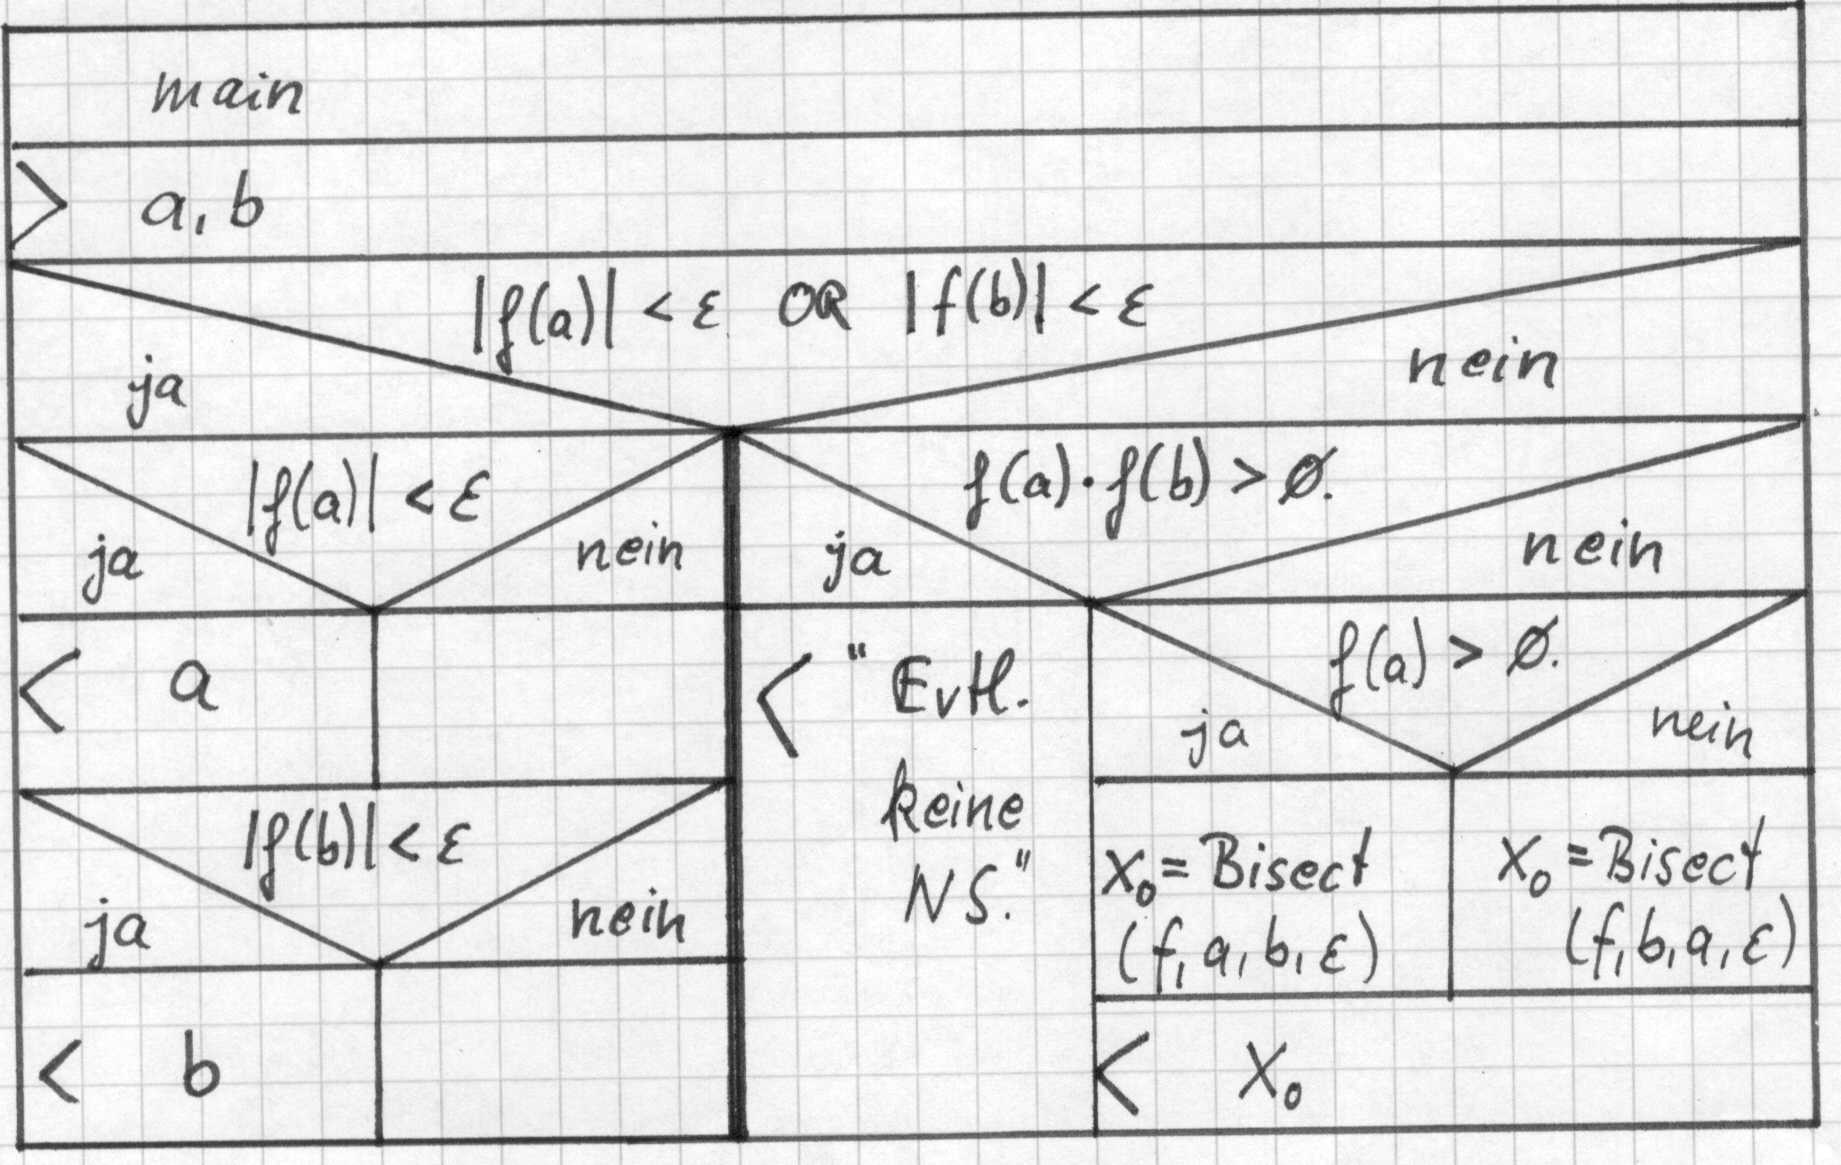
\includegraphics[scale=0.7]{GIF/p88}


Als kr"onenden Abschlu"s definieren wir uns im Programm weitere Funktionen
$h(x)=3-e^x$, $t(x)=1-x^2$, fragen den Nutzer welche math.\  Funktion
f"ur die Nullstellensuche benutzt werden soll und berechnen
die Nullstelle(n) im gegebenen Intervall.
Diese Auswahl kann leicht mit einer \verb|switch|-Anweisung realisiert werden und
f"uhrt zu Version~V des Programmes.
%\bspfile{Bisect5.cpp}
%\includecode[linerange={12-12,30-33,39-40,51-51,64-64,73-73,106-106,112-113}]{Bisect5.cpp}{Bisektion-V mit einer Funktionvariablen}
\includecode[linerange={11-11,30-40,51-51,64-64,107-107,112-113}]{Bisect5.cpp}{Bisektion-V mit einer Funktionvariablen} 

\underline{Bemerkung:}
Die drei Funktionen \verb|Bisect|[1-3]() unterscheiden sich in ihren
Parameterlisten. Deshalb k"onnen alle drei Funktionen unter dem Namen
\verb|Bisect()| verwendet werden, da sich ihre Signaturen unterscheiden
und somit der Compiler an Hand der Parameterliste genau wei"s, welche Funktion \verb|Bisect()|
verwendet werden soll.\index{Funktion|)}
\bspfile{Bisect6.cpp}\index{Bisektion|)} 
%
%
%

Statt der gesonderten Dekalaration einer globalen Funktion können wir statt \verb|ff| oder \verb|t| 
gleich den kurzen Funtionscode als Lamda-Funktion (siehe~\S\ref{p:11.2.1.4}) übergeben:
\bspfile{../SS24/Bisect/Bisect3_lambda.cpp}
%\\
%%
%\verb|    x0 = Bisect( [ ] (const double x) {1-x*x;}, a, b, EPS );|
%\\
\begin{lstlisting}[caption=Lambda-Funktion in Bisect,label=lst:7_9_18,basicstyle=\scriptsize]{}
    x0 = Bisect( [ ] (const double x) {1-x*x;}, a, b, EPS );
\end{lstlisting}






